
\begin{figure}[!ht]
    \centering
    \subfloat[Close Set Domain Adaptation (\textbf{CSDA})]{
        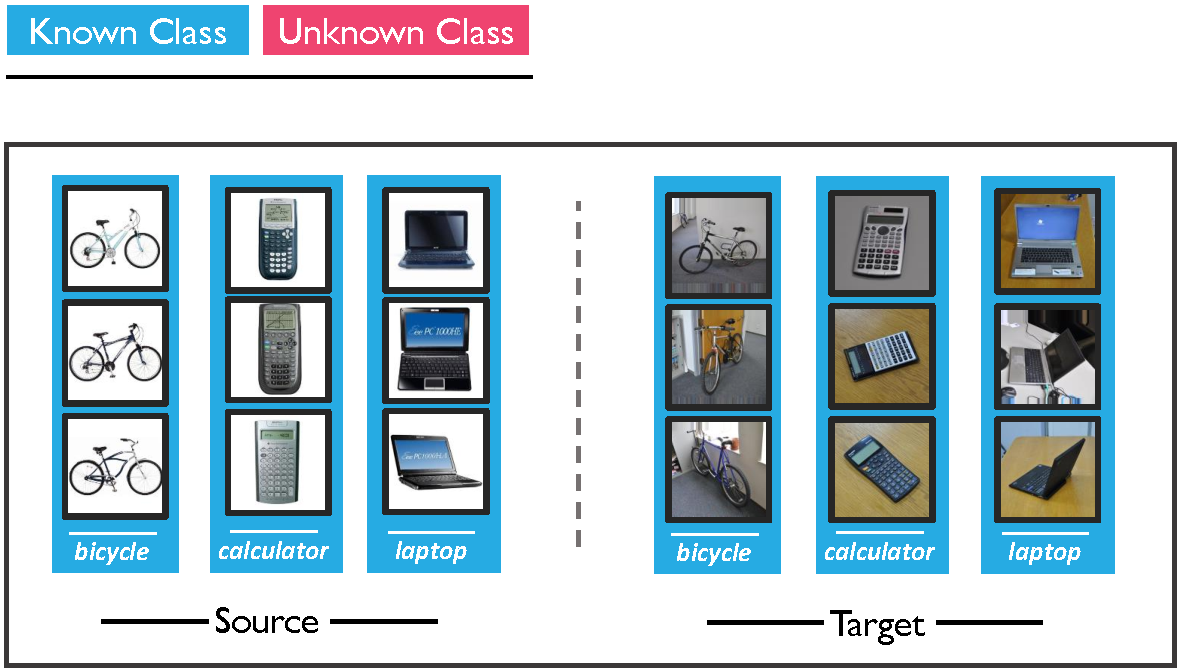
\includegraphics[width=0.48\textwidth]{contents/figures/pdf/closeset.pdf} 
        \label{figure: CSDA}
    } \\
    % \hfil
    \subfloat[Open Set Domain Adaptation (\textbf{OSDA})]{
        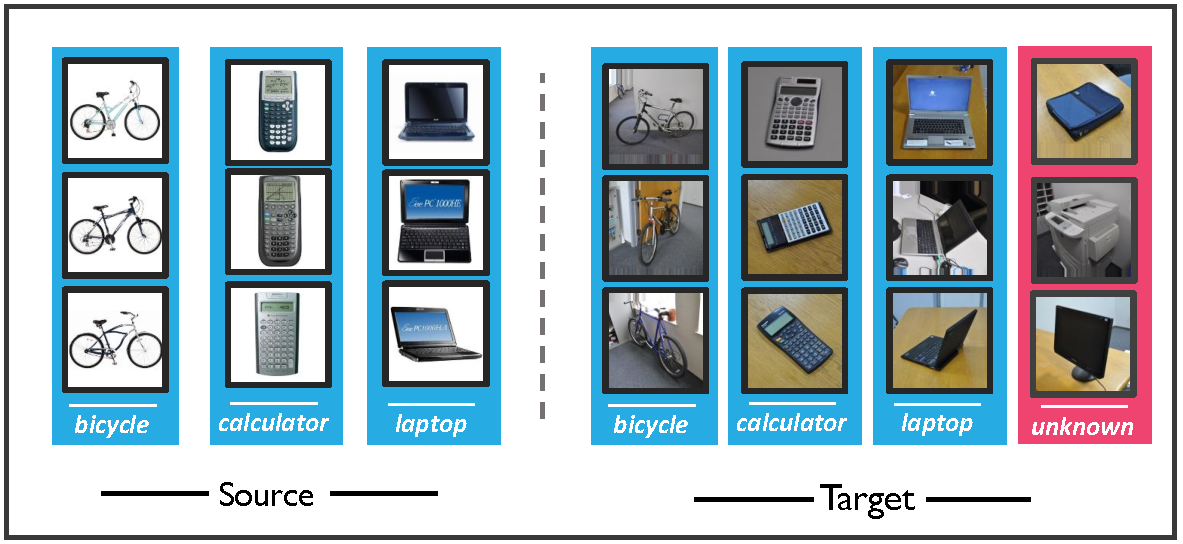
\includegraphics[width=0.48\textwidth]{contents/figures/pdf/openset.pdf} 
        \label{figure: OSDA}
    }
    \caption{
        A comparison between close set domain adaptation and open set domain adaptation that we follow. 
        (\textbf{a}): The close set domain adaptation setting used in most work where source domain and target domain has the same label space. 
        (\textbf{b}): The openset domain adaptation setting proposed in \cite{OpensetDA-bp} which is more challenging and realistic scenario. In such setting, the target label space subsumes the source label space, the unknown class samples in target domain will cause negative transfer.
    } 
    \label{figure: openset} 
\end{figure}

